%%%%%%%%%%%%%%%%%%%%%%%%%%%%%%%%%%%%%%%%%%%%%%%%%%%%%%%%%%%%%
%% HEADER
%%%%%%%%%%%%%%%%%%%%%%%%%%%%%%%%%%%%%%%%%%%%%%%%%%%%%%%%%%%%%
\documentclass[a4paper,oneside,12pt]{report}

%% Language %%%%%%%%%%%%%%%%%%%%%%%%%%%%%%%%%%%%%%%%%%%%%%%%%
\usepackage[english]{babel}
%\usepackage[greek]{babel}
%\usepackage[utf8x]{inputenc}
\usepackage{lmodern} %Type1-font for non-english texts and characters
\usepackage[ansinew]{inputenc}
\usepackage[T1]{fontenc}
%\usepackage{kerkis}

%% Formatting %%%%%%%%%%%%%%%%%%%%%%%%%%%%%%%%%%%%%%%%%%%%%%%
\frenchspacing
\usepackage{parskip}
%\usepackage{fullpage}
\usepackage{a4wide}
%\usepackage{setspace}
\usepackage{titlesec} % Package to allow chapter number on the same line as chapter title
\titleformat{\chapter}[hang]  % Package to allow chapter number on the same line as chapter title
{\normalfont\huge\bfseries}{\chaptertitlename\ \thechapter:}{0.5em}{\filright} % Package to allow chapter number on the same line as chapter title

\usepackage{subfig}

%% Bibliography management % % % % % % % % % % % % % % % % %
%\usepackage[backend=bibtex, style=numeric]{biblatex}

%% Packages for Graphics & Figures %%%%%%%%%%%%%%%%%%%%%%%%%%
\usepackage{graphicx}
\usepackage[section]{placeins}
\usepackage{float}
\restylefloat{table}
%%Float Adjustment
%two column float page must be 90% full
\renewcommand\dblfloatpagefraction{.90}
%two column top float can cover up to 80% of page
\renewcommand\dbltopfraction{.80}
%float page must be 90% full
\renewcommand\floatpagefraction{.90}
%top float can cover up to 80% of page
\renewcommand\topfraction{.80}
%bottom float can cover up to 80% of page
\renewcommand\bottomfraction{.80}
%at least X% of a normal page must contain text
\renewcommand\textfraction{.1}
%separation between floats and text
\setlength\dbltextfloatsep{9pt plus 5pt minus 3pt }
%separation between two column floats and text
\setlength\textfloatsep{4pt plus 2pt minus 1.5pt}
\usepackage{tikz}
\usetikzlibrary{arrows, shapes, automata,petri}

%% Math Packages %%%%%%%%%%%%%%%%%%%%%%%%%%%%%%%%%%%%%%%%%%%%
\usepackage{amsmath}
\usepackage{amsthm}
\usepackage{amsfonts}
\usepackage{bm}
\DeclareMathOperator{\Cov}{Cov}
\DeclareMathOperator{\Var}{Var}
\usepackage[retainorgcmds]{IEEEtrantools}

%% Packages for document interactivity
\usepackage{hyperref}
\hypersetup{
		colorlinks,
    citecolor=black,
    filecolor=black,
    linkcolor=black,
    urlcolor=black
}
\usepackage{url}
\usepackage[nottoc]{tocbibind} % Add the bibliography in the ToC

%% Other options to examine %%%%%%%%%%%%%%%%%%%%%%%%%%%%%%%%%
%\usepackage{usenames, dvipsnames]{color}
%\usepackage{amssymb}
%\usepackage{cclicenses}
%\usepackage{siunitx}
%\usepackage{ucs}
%\raggedbottom
\newcommand{\HRule}{\rule{\linewidth}{0.5mm}}
%\renewcommand{\labelenumi}{\roman{enumi}}
%\usepackage{sinunitx}

% % % % % % % % % % % % % % % % % % % % % % % % % %
% % BIBLIOGRAPHY
% % % % % % % % % % % % % % % % % % % % % % % % % % %
%\addbibresource[label=biblocal]{References.bib}
%\addbibresource[label=uavModeling]{../UAV\ Modelling/References.bib}

%%%%%%%%%%%%%%%%%%%%%%%%%%%%%%%%%%%%%%%%%%%%%%%%%%%%%%%%%%%%%
%% DOCUMENT
%%%%%%%%%%%%%%%%%%%%%%%%%%%%%%%%%%%%%%%%%%%%%%%%%%%%%%%%%%%%%
\begin{document}

\pagestyle{empty} %No headings for the first pages.


%% Title Page %%%%%%%%%%%%%%%%%%%%%%%%%%%%%%%%%%%%%%%%%%%%%%%
\begin{titlepage}
\begin{center}
\includegraphics[width=0.3\textwidth]{./ntua_logo}~\\[1cm]

\HRule \\
\linespread{1.5}
\begin{huge}
%% Title Section %%
Integrating Fault Detection and Diagnosis into Fixed-Wing UAVs \\
\end{huge}
\begin{LARGE}
PhD Research Documentation
\par
\end{LARGE}
\HRule \\

\vfill

{\Large
%% Author %%
Georgios Zogopoulos - Papaliakos
} \\[0.3cm]
\textsc{\large 
%% Company %%
National Technical University of Athens
}\\
\textsc{School of Mechanical Engineering\\ Control Systems Laboratory} \\[0.3cm]
e-mail: \texttt{
%% E-mail address
gzogop@mail.ntua.gr
} \\[1cm]
{
%% Location %%
Athens
, \today}

	

 %\thanks{
  %\textlatin{This work is licenced under} \href{http://creativecommons.org/licenses/by-nc/4.0/deed.el}
  %{\emph{\textlatin{Creative Commons Attribution-NonCommercial 4.0 Greece License}}}
\end{center}
%\maketitle

\end{titlepage}

%% Dynamic Content %%%%%%%%%%%%%%%%%%%%%%%%%%%%%%%%%%%%%%%
%% The Table of Contents
\tableofcontents 
\pagestyle{plain} %Now display headings: headings / fancy / ...

%% The List of Figures
%\clearpage
%\addcontentsline{toc}{chapter}{List of Figures}
%\listoffigures

%% The List of Tables
%\clearpage
%\addcontentsline{toc}{chapter}{List of Tables}
%\listoftables

\clearpage

%%Main Body %%%%%%%%%%%%%%%%%%%%%%%%%%%%%%%%%%%

\renewcommand{\chaptername}{} % Suppress the phrase "Chapter #" at the beginning of every chapter
%\renewcommand{\thechapter}{} % Suppress chapter numbering

\nocite{*} % Add uncited bibliography to the bibtex database

%\pagestyle{myheadings}

\chapter{Why Do UAVs Need FDD Systems}

Aerial robotic systems, also known as Unmanned Aerial Vehicles (UAVs) are becoming increasingly popular during the past decade. After seminal research on military applications ran its lifespan, smaller and less expensive systems found their way to research institutes globally. After the imperative and necessary control problems where solved and structural designs where streamlined, UAVs finally found their way to the consumer at the end of the 2000's, as a natural extension of the radio-controlled aircraft market.

The public quickly embraced this new technology and as of 2014, consumer Unmanned Aerial Systems (UASs) are widely used for aerophotography, ground surveys and recreation. However, the fact that UAVs are able to pilot themselves using well-established control algorithms for the nominal case, does not mean that they are able to remain operational in case of faults. Indeed, amateur UAV operators rarely perform Standard Operational Procedures, pre-flight checks or pre-emptive maintenance. As a result, the sight of a UAV falling out of the sky is all too common.

One would argue that operators should be the ones responsible for correct system practices, situation assessment and integrity checks. However, every time a technology gains wide acceptance to the public, eventually the task of safety assurance falls onto the manufacturer. As a comparison, consider how common and indispensable safety systems such as the ABS, ESP and vehicle diagnostics are in the automotive industry. If consumer UAVs are to become a part of our everyday lives, have a respectable degree of reliability and conquer the skies, safety standards must be built at the system level. This is the objective of the discipline of Fault Detection and Diagnosis (FDD)

Let us loosely describe Fault Detection and Diagnosis here and provide a more rigorous, mathematical definition later. Faults are events that throw a system out of its nominal mode of operation. Most of the times, faults, if allowed to go unchecked, will eventually result to system failures, which is an unwanted situation. Hence, it is of our interest to detect faults at their birth and take counter-measures against them, in order to ensure system health and if possible, maintain its operational status. Fault Detection involves setting up mathematical and physical structures that are able to detect when a fault occurs in our system. Afterwards, Fault Isolation should be performed, in order to identify the system component which is under fault. This is an important piece of information, since it allows us to target the source of a fault and is a necessary prerequisite for reconfigurable, fault-tolerant control (FTC). Finally, Fault Detection methods allow us to assess the magnitude of the fault, be it the drift of a physical parameter value, the flow of a leak or the strength of a disturbance. Oftentimes, Isolation and Detection are mutually referred to as Diagnosis.

 % Need of FDD
\chapter{Historical FDD Overview}

Fault Detection and Diagnosis is a subject of research since the end of the 70's, originally intended for application in the petrochemical industry, which was a very innovative, wealthy and large-scale sector at that time. Employing mainly state and parameter estimation techniques, which where very costly computationaly-wise at the time, FDD was barely applicable to the slow-evolving chemical processes.

During the 90's, when adaptive control was a new topic of interest, FDD was re-visited to aid in building fault-tolerant control systems. Especially in the airline industry, which at that time was both booming and employing in-flight computers with system-wide span, efforts where made to design systems which would automatically intervene to the pilot's actions, to detect some basic faults and avert potential (and potentially very expensive and life-threatening) accidents. However, the costly experimental iterations, as well as the inability to guarantee the correct operation of the fault-tolerant control system, which would in turn jeopardize human lives, prevented FDD and FTC from reaching their full potential in airborne systems.

UAVs provide the low-cost and disposable test platform which is needed to verify the efficiency of FDD methods and are getting increasing interest with every successful research milestone. % 
\chapter{The Current FDD Scope w.r.t. Fixed-Wing UAVs}

The most fatal failure on a fixed-wing UAV (which have the traditional "airplane" shape), apart from severe structural damage, is a malfunction of its control surfaces. Indeed, an airplane could perform an emergency landing with malfunctioning undercarriage, with a reduced sensor suite, with a broken propeller or even without an engine. But without properly functioning ailerons and elevators the aircraft is essentially crippled. This is why most research in fw-UAV FDD revolves around detection of faults of control surfaces and their corresponding actuators.
Other research topics include detection of Pitot tube malfunctions and icing scenarios. The latter does not directly apply to consumer-grade UAVs, as the icing phenomenon occurs in high altitudes and low temperatures. The former has indeed applicable results to all fw-UAV airframes.
\chapter{The Need for Holistic System Health Monitoring}

As is often quoted "The whole is more than the sum of its parts". In the case of fw-UAVs, the low-level system components have attributes and effects which not only affect themselves or the components they are connected to, but also the subsystem they belong to or even the whole airframe. Electrical, mechanical and dynamic interdependencies between components form a mesh of interactions, the knowledge of which is valuable. Each component is not isolated; its faults affect other parts of the system, even beyond its subsystem, and in turn said component may depend on other components working properly for itself to operate nominally. As an example, consider the case of an electric UAV, where a part of the propeller blade gets clipped, as a result of a hardware failure. Immediately, because of the imbalanced load on the motor shaft, the propeller angular inertia is increased and the motor struggles to maintain its commanded RPM. This results in excessive current draw and also reduced thrust power. Moreover, vibrations are generated and transmitted throughout the airframe, cluttering the accelerometer sensor bandwidth and possibly affecting the autopilot performance. Even in simple, single-component failures, the implications on a fast-evolving, tightly-coupled system may be severe and in ways that may not be directly apparent or so complex that are difficult to keep track of.

To showcase the extent of the problem, an indicative list of an UAV system resources and potential failures is presented.

\begin{table}[rc]
%\centering
\begin{minipage}[t]{0.45\textwidth}
\vspace{0pt}
\begin{tabular}{l}
{\textbf{System Resources}}\\
\hline
\underline{Hardware} \\
motor \\
actuators \\
sensors \\
video \& data tranceivers \\
antennae \\
fuel\\battery capacity \\
processing units (on-board computers) \\
aerodynamics surfaces \\
structural support \vspace{5pt}\\

\underline{Software} \\
Computational power \\
Computational memory \vspace{5pt} \\
\underline{Other}\\
Airspeed \\
Altitude
\end{tabular}
\end{minipage} %
%
\begin{minipage}[t]{0.45\textwidth}
\vspace{0pt}
\begin{tabular}{l}
{\textbf{System Faults}}\\
\hline
\underline{Hardware} \\
propeller damage \\
propeller dislocation \\
motor loss of power \\
motor total failure \\
power supply cut-off \\
power supply total failure \\
battery shortened life \\
battery fire \\
actuator failure \\
control surface dislocation\\
control surface break-off\\
sensor elevated noise floor \\
sensor failure\\
communication partial/total loss\\
structural failure partial/total\\
aerodynamic surface alteration\\
center of gravity dislocation \\
processor damage \vspace{5pt}\\
\underline{Software}\\
bugs\\
unexpected states
\end{tabular}
\end{minipage} %

\end{table}

It is apparent that in order to investigate the dependencies between system resources and system faults, with regard to component descriptions, we need to handle the system complexity using a formal, scalable representation method for this kind of dependencies.
\chapter{Tackling System Complexity}

\section{Component Model}

An effort to describe the system structure in a well-defined and scalable way will now be made. The core building block is the component, which will be subsequently defined. To better illustrate our approach, the example of a 1-axis digital MEMS gyroscope will be presented alongside the definition.

Initially, the notion of the service will be introduced. A service is a 6-tuple of the form:

\quad <consumed variables, produced variables, procedure, request, activation condition, resources>

This model describes the service as a process which uses \textit{consumed variables} upon \textit{request} according to a \textit{procedure} in order to return \textit{produced variables}. In order for the service to be carried out \textit{resources} are used up and an \textit{activation condition} must hold true.

Thus, using set theory for every mentioned quantity, we can define a set of services provided by a component k as:

\textbf{Definition: Service}
\begin{align*}
S(k) &= \left\{s_i(k),i\in I_s(k)\right\} \\
s_i(k) &= \left\{cons_i(k),prod_i(k),proc_i(k),rqst_i(k),active_i(k),res_i(k)\right\}
\end{align*}

The set $I_s(k)$ contains the service indices which are applicable to the component k. The same holds for the sets $cons(k),prod(k),proc(k),active(k),res(k)$.

In the case of the MEMS accelerometer with the component index 1, we can define:
\begin{align*}
I_s(1) &= \left\{1,2\right\} \\
cons(1) &= \left\{\text{angular rate }\omega, \text{temperature }K, \text{measurement noise }w, \text{initial angle input }\theta_{0i}\right\} \\
prod(1) &= \left\{\text{measured angular rate }\omega_m, \text{measured angle }\theta_m\right\} \\
proc(1) &= \left\{ \omega_m = \omega + c_1K + w, \theta_m = \theta_0 + \int\omega_m, \theta_0 = \theta_{0i}\right\} \\
rqst(1) &= \left\{ \text{I2C command}\right\} \\
active(1) &= \left\{ \text{Power supply present}\right\} \\
resources(1) &= \left\{ \text{current consumption rate}, \text{gyroscope unit}, \text{I2C channel}\right\} \\
S(1) &= \left\{s_1(k),s_2(k)\right\}
\end{align*}
Where service $s_1(1)$ is the initial sensor angle specification and $s_2(1)$ is the measurement of angular rate and angle.

\textbf{Definition: Use Mode}
We define a set of use-modes
\begin{align*}
M(k) &= \left\{m_i(k), i\in I_m(k)\right\} \\
\end{align*}
where $m_i(k)$ is the set of indices of the available component k services during the use mode i and $I_m(k)$ is the set of indices of available use modes for the component k. The applicability of services during a use mode is a designer choice.
In our example we have two use modes:
\begin{align*}
m_1(1) &= \left\{s_1(1)\right\} \quad \text{calibration mode}\\
m_2(1) &= \left\{s_2(1)\right\} \quad \text{operational mode}
\end{align*}

\textbf{Definition: Component Model}
We are now finally able to define a component as the aggregation:
\begin{align*}
\text{<component k>} &\equiv \text{<state transition graph }G(M(k),\tau(k),m^0(k))> \\
<M(k)> & \\
<\tau(k)> & \\
<m^0(k)> & \\
<m_i(k)> & \\
<s_i(k)> & \\
\end{align*}

\section{Structural Model}

Given the component descriptions we have set up and their interconnections, we can "translate" the component behavioural model onto a qualitative model for structural analysis. The qualitative model retains data only about the information flow and the component interconnections. It is essentially a directional graph which visualizes the evolution of the variables from the known system inputs towards the also known system outputs, via the unknown system internal variables and states.

A vital definition towards this goal is that of the \textit{constraint}. A constraint is a relation between two system variables, which expresses a physical model, a component model or a control law. In essence, the sum of the system constraints constitutes the full set of equations, either algebraic or differential, which make up our system.

Based on the previous component definition, the system constraints are the union of the component procedures
\begin{align*}
\mathcal{C } &= \bigcup proc(k)
\end{align*}

while all the variables involved in $\mathcal{C}$ constitute the variable set $\mathcal{Z}$.

Variables whose values are known (inputs, measurements etc) belong to the known variables set $\mathcal{K}$, whereas the rest of the variables belong to the unknown variables set $\mathcal{X}$. It holds that $\mathcal{Z = K \cup X}$.

We define a bi-partite graph ($\mathcal{C, Z, A}$), with vertices $\mathcal{C, Z}$ and edges $\mathcal{A}$ linking constraints with their corresponding variables.
It is meaningful to define directionality in the graph, to reflect the fact that a single constraint cannot be solved for any of its variables. Indeed, from the simple differential equation $x_2 = \dot{x_1}$, we cannot extract the values of $x_1$, since that would require the additional initial condition, which is not given.

An important segmentation of $\mathcal{C}$ in regard to $\mathcal{Z}$ is splitting it to:\\
$\mathcal{C_K}$, which contains the restrictions which refer only to known variables\\
$\mathcal{C_X}=\mathcal{C-C}_K$

To showcase this approach, let us consider another example, a spring-mass system with position measuring.
\begin{alignat*}{2}
c_1: &\quad& \dot{x} &= \frac{d}{dt}x \\
c_2: &\quad& v &= \dot{x} \\
c_3: &\quad& \dot{v} &= \frac{d}{dt}v\\
c_4: &\quad& \dot{v} &= \frac{K}{m}x\\
m_1: &\quad& x_m &= x\\
\end{alignat*}

The constraints set is $\mathcal{C}=\left\{c_1, c_2, c_3, c_4, m_1\right\}$\\
The known variables set is $\mathcal{K}=\left\{x_m\right\}$\\
The unknown variables set is $\mathcal{X}= \left\{x, \dot{x}, v, \dot{v}\right\}$\\
The resulting graph is: \\
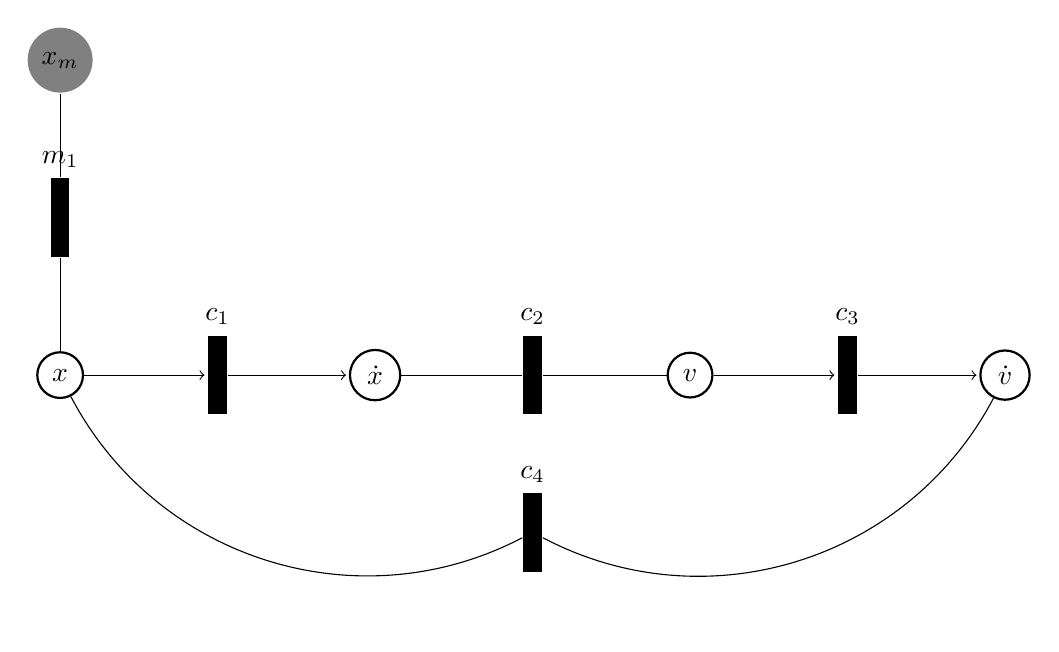
\begin{tikzpicture}[node distance = 2cm, bend angle=45, auto]
\tikzstyle{known_var}=[circle, thick,fill=gray]
\tikzstyle{unkno_var}=[circle, draw=black, thick]
\tikzstyle{constr}=[rectangle, fill=black, thick, minimum height=10mm, minimum width = 1mm]
%
\begin{scope}

\node [known_var] [](xm) {$x_m$};
\node [constr] (m1) [below of=xm,label=$m_1$] {}
	edge [] (xm);
\node [unkno_var] (x) [below of=m1] {$x$}
	edge [] (m1);
\node [constr] (c1) [right of=x, label=$c_1$] {}
	edge [pre] (x);
\node [unkno_var] [right of=c1](xdot) {$\dot{x}$}
	edge [pre] (c1);
\node [constr] [right of=xdot, label=$c_2$] (c2) {}
	edge [] (xdot);
\node [unkno_var] [right of=c2] (v) {$v$}
	edge [] (c2);
\node [constr] (c3) [right of=v, label=$c_3$] {}
	edge [pre] (v);
\node [unkno_var] [right of=c3] (vdot) {$\dot{v}$}
	edge [pre] (c3);
\node [constr] [below of=c2, label=$c_4$] (c4) {}
	edge [bend right] (vdot)
	edge [bend left] (x);

\end{scope}
%
\end{tikzpicture}

Naturally, this graph could be represented as an incidence matrix $D$, where $$
d_{ij} = \left\{\begin{array} {rl}
0 \quad &\text{if }(z_i, c_i)\in\mathcal{A} \\
1 \quad &\text{if }(z_i, c_i)\notin\mathcal{A} 
\end{array}\right.
$$
We could extend this definition to include the graph directionality if we wanted to, by setting the vertices of $\mathcal{A}$ to not be bi-directional but rather two separate vertices. This would make the matrix D non-symmetrical.

Having set up the necessary mathematical tools (graphs and adjacency matrices) to explore the system structure, we are able to gain much more insight on our system. For example, we can use the existence of paths connecting nodes to explore whether one variable $ x_1$of our system is related to another $x_2$, in other words, if $\frac{\partial}{\partial x_1}x_2 \neq 0$.
Moreover, we can discuss about whether an internal variable is \textbf{observable}, by finding connected paths originating from it and reaching known variables. Finally, we can even find if variables of our system are \textbf{controllable}, by looking for connected paths to input variables. This will be especially useful in cases where we want to design reconfigurable controllers for our system.

\chapter{The Matching Problem}

In the previous chapter, we saw how the system model structure can be represented in a qualitative way by using bi-partite graphs. Using this information, we need to acquire a way, ie a computation sequence, which will allow us to calculate the unknown variables in $\mathcal{X}$ from the inputs and measurements in $\mathcal{K}$. It goes without saying that such a calculation sequence cannot be derived by hand in large-scale systems. Actually, the problem of calculating each element from the set $\mathcal{X}$ using an element from $\mathcal{K_X}$ only once can be generalized to a common problem in graph theory, called \emph{the matching problem} \cite[ch~26]{Leiserson2009}.

Given a graph $G=(V,E)$, a \textbf{matching} is a subset $M\subseteq E$ such that for all vertices $v \in V$, at most one edge of $M$ is incident on $v$. We say that $v$ is matched by the matching $M$ if an edge of $M$ is incident on $v$. A \textbf{maximum matching} is a matching with maximum cardinality for a particular graph. A maximum matching is not necessarily unique. We say that a matching is complete in $V$ if $\left|M\right|=\left|V\right|$.

\section{Matchings in Bi-Partite Graphs}

In the case of a bipartite graph $G = (C,X,E)$, where $C$ is the set of constraints, $X$ the set of unknown variables and the edge set $E$ connects the variables to the constraints they appear in, the matching problem can be elaborated a bit more. For a given bi-partite graph, a matching may be complete either in $\mathcal{C}$, or in $\mathcal{X}$, or both or neither.

The following figure presents various matching for a bi-partite graph:
\begin{figure}[H]
\centering
\includegraphics[width=0.7\linewidth]{Figures/matching}
\caption{Matchings on a bi-parite graph}
\label{fig:bipariteMatching}
\end{figure}

In the first and second subfigure we see incomplete matchings on the graph, both in terms of $L$ and $R$. However, the second matching is maximum, since no matching with greater cardinality can be found in this graph.

We can interpret the notion of matching for our need to solve the structural graph as follows: if a variable $x \in \mathcal{X}$ is matched with a vertex $e \in M$, then we also say that it is matched to the constraint $c \in \mathcal{C}$ which $e$ is incident onto, ie $(c,x) \in M$. This can be further extended to say that we can \textbf{calculate} $x$ by using $c$. Hence, no other variable can be calculated using $c$ and no other constraint can produce $x$.

The above interpretation applies a directionality in the bipartite graph. Let $E'$ be a new edge set where 
\begin{equation} \label{eq:matchedDirGraph}
E' = \left\{(c,x) \in E : (c,x) \in M\right\} \cup \left\{(x,c) \in E : (x,c) \notin M\right\}
\end{equation}

Through the procedure of matching, a new directed graph $G'=(C,X,E')$ is produced whose direction dictates the calculation order of the model structure and visualizes the information flow. 
\begin{itemize}
\item if an edge connects a constraint to a variable, then this variable is calculated using this constraint.
\item if an edge connects a variable to a constraint, then this variable is used by this constraint.
\end{itemize}

Paths are created, which connect variables as they contribute to the calculation of other variable, down the path.

\section{Constraints in Matchings of Graphs Representing Real-World Systems}

The matching process works very efficiently and without problems in undirected graphs. However, in bi-partite structural graphs resulting from real-world systems many problems arise, which restrict the feasibility of a complete matching in $\mathcal{X}$ and make the matching process difficult.

Notice how in (\ref{eq:matchedDirGraph}) the directionality of each edge $e \in E$ is respected. We cannot match $c$ to $x$ ($(c,x) \in M$) if $(c,x) \notin E$. Similarly, we cannot expect a variable $x$ to be used by a constraint $c$ if $(x,c) \notin E$.

Another problem arises from the fact that there is no guarantee that the calculation process created by a matching and the corresponding directional graph can be back-tracked only to known and or measured variables, ie in the transpose graph $G'\top$ there is always a path from $x \in \mathcal{X}$ to $\mathcal{K}$. This leaves us with an incomplete calculation sequence which has unknown variables as input. In the general approach, the only way to verify the feasibility of the calculation sequence is to test if $\mathcal{X}$ is \textbf{reachable} from $\mathcal{K}$ in $G'$.

Moreover, $G'$ is not guaranteed to be acyclic. The existence of cycles in $G'$ is equivalent to the presence of systems of equations in the calculation sequence which have to be solved simultaneously. Since the constraints involved are not necessarily linear and may also be differential, systems of \textbf{ordinary differential equations} or even \textbf{differential algebraic equations} may need to be solved in real-time in order for the sequence to be calculable. Depending on our assumptions, this may or may not be feasible. Initial conditions may be unknown or the mathematical and numerical tools to solve such systems may not be available to the monitoring system. Hence, we may want to mark such loops as incalculable and restrict the calculation sequence beyond them.

Finally, we may want to favour some matchings over others. Reasons to do this are to avoid too many differentiations in the calculation sequence which enhance the noise or avoid solving a constraint in terms of a variable to which the constraint has small sensitivity or high cost of implementation.

Examples for the second case are the constraints
\begin{IEEEeqnarray}{lrCl}
e_1: & x_1 + \sin x_2 &= &0 \IEEEyesnumber \IEEEyessubnumber\\
e_2: & x_1^2 + x_2 &= &0 \IEEEyessubnumber \\
e_3: & x_1 + 0.0001 x_2 + 10 x_3 &= &0 \IEEEyessubnumber
\end{IEEEeqnarray}

\begin{itemize}
\item We would prefer solving $e_1$ for $x_1$ rather than for $x_2$, since the sensitivity of $e_1$ to $x_2$ for $x_2$ around $\pi/2$ becomes 0.
\item We would prefer solving $e_2$ for $x_2$ for $x_2$ rather than from $x_1$, since calculating the power of 2 is cheaper than calculating a square root.
\item Assuming comparable variable orders of magnitude, we would prefer solving $e_3$ for $x_1$ or $x_3$ rather than for $x_2$, since $e_3$ is much more sensitive to noise in $x_1$ and $x_3$ in contrast to noise from $x_2$.
\end{itemize}

The following example demonstrates how the above constraints affect the selection of the appropriate matching.

We are given the system
\begin{IEEEeqnarray}{lrCl}
c_1: & x_1 - 100 u_1 &= &0 \IEEEyesnumber \IEEEyessubnumber\\
c_2: & 3 x_4 + 7 x_2 - x_1 + x_5 &= &0 \IEEEyessubnumber \\
c_3: & 5x_2 - x_3&= &0 \IEEEyessubnumber \\
c_4: & 10x_3 + 4x_4 &= &0 \IEEEyessubnumber \\
c_5: & x_8 - 2x_7 - x_5 &= &0 \IEEEyessubnumber \\
c_6: & x_8 - \frac{d}{dt}x_7 &= &0 \IEEEyessubnumber \\
c_7: & x_9 \cdot x_1 -1 &= &0 \IEEEyessubnumber \\
c_8: & x_6 - x_9 &= &0 \IEEEyessubnumber \\
c_9: & y_1 - \frac{d}{dt}x_9 &= &0 \IEEEyessubnumber \\
c_{10}: & x_5 - x_6^3 + 1 &= &0 \IEEEyessubnumber \\
c_{11}: & x_5 + x_1^{1.5} &= &0 \IEEEyessubnumber
\end{IEEEeqnarray}

The structural graph of the system is depicted below.

\begin{figure}[H]
\centering
\includegraphics[width=0.7\linewidth]{Figures/unmatchedConstrGraph}
\caption{The bi-parite graph of the previous system}
\label{fig:matchingConstraints}
\end{figure}

Notice how the causality of some equations pre-enforces directionality on some of the edges:
\begin{itemize}
\item Known variables (inputs and measurements, shown in green) can only be used as inputs in the constraints, not calculated by them.
\item Variables differentiated in time can only be used as input to constraints, due to derivative causality (eg in $c_6$).
\end{itemize}

A good matching on the above graph is shown below. The edges which belong to the matching are emphasized and the rest of the edges are directed in such a way so as the matching is respected. We verify that at most one edge leaves a constraint vertex and at most one edge enters a variable vertex.

\begin{figure}[H]
\centering
\includegraphics[width=0.7\linewidth]{Figures/matchedConstrGraph}
\caption{A matching of the structural graph with desirable properties}
\label{fig:matchingConstraints}
\end{figure}

The above matching has some very desirable properties:
\begin{itemize}
\item It is a maximum matching on the varables set.
\item The each edge of the resulting directed graph respects the directionality of the original graph.
\item When possible, the least expensive calculation is selected, as in the case of $x_6$, which is calculated through $c_8$, rather than $c_{10}$
\end{itemize}

Naturally, the existence of loops in the resulting directed graph cannot be avoided, since this is a property of this particular, actual, real-world system. Whether it is possible to solve them depends on the available analytical and numerical tools we have.

\chapter{Uncovering Analytical Redundancy}

A common tool which Fault Tolerant Control uses in order overcome faults and failures is \textit{redundancy}. System components redundant to each other offer the same functionality with regard to an objective. They may operate simultaneously and cooperatively, or they might only perform a hand-over of the objective in the case where one of them fails. \textit{Hardware redundancy} is about including multiple hardware components to assure that within the pre-specified Mean Time Between Failures (MTBF) the overall system will have at least one component to carry out each necessary objective. Hardware redundancy in fw-UAVs is most prevalent in the form of duplicate sensors or actuators.
However, there is another form of redundancy, \textit{analytical redundancy}. This is about surplus of signal information. If our system structure contains more constraints than variables, ie $ |\mathcal{C}|<|\mathcal{Z}|$, then the system is called \textbf{over-constrained}. In the case of sensor redundancy, there is more than one way (path) to observe (connect) some variables from already known variables, thus removing the need for an extra hardware sensor. In the case of actuator redundancy, uncovering redundancy of an output signal against input signals makes it obvious that there is more than one way to affect the specific output variable, thus alleviating the need for a redundant actuator.
Given the nature of small-scale UAVs, it is very desirable to keep their cost and weight to a minimum. Hence, our goal is to find ways to replace hardware redundancy with analytical redundancy, as much as possible.

\section{Solving the System Graph}

One of the most useful ways one can employ system structural analysis, is indeed to uncover methodically such redundancies within a large-scale system. Instrumental to this goal is the notion of graph matching.

\textbf{Definition: Matching}\\
A matching $\mathcal{M}$ is a subset of $\mathcal{A}$ such that the restrictions of the projections $p_\mathcal{C}$ and $p_\mathcal{Z}$ to $\mathcal{M}$ are injective.\\
\begin{math}
\forall e_1,e_2 \in \mathcal{A} : e_1 \neq e_2 \Rightarrow p_\mathcal{C}(e_1) \neq p_\mathcal{C}(e_2) \wedge p_\mathcal{Z}(e_1) \neq p_\mathcal{Z}(e_2)
\end{math}

This means that given the set of edges $\mathcal{A}$, we select edges so that no two edges have a common vertex. If the cardinality of $\mathcal{M}$ is the maximum possible for a given  $\mathcal{A}$, then the matching is called \textbf{maximal}. If  $\mathcal{M}$ covers all the variables, then it is called \textbf{complete} with respect to  $\mathcal{Z}$

By using the notion of matching, given a system graph, we can reveal analytical redundancy locations, in the form of unmatched constraints. These can be used to "double-check" the correct operation of our system. The difference of the LHS and RDS of an unmatched constraint equation is called a \textbf{residual}. Under nominal system operation all residuals evaluate to zero. If a system constraint is altered, then the unmatched constraint will no longer hold and the associated residual will deviate from zero.

For the previous example of the spring-mass system, a possible complete matching is:
\input{graphMatch}

The matching set is $\mathcal{M}=\left\{(m_1,x),(c_1,\dot{x}),(c_2,v),(c_4,\dot{v})\right\}$. The matched edges are denoted in the graph in bold.

Notice that the matching is complete in respect of the variables and incomplete in respect to the constraints. That leaves room for one residual generator at the node of $c_3$.
The way we can take advantage of the matching is to evaluate the variables adjacent to the unmatched constraint through the given matching and then evaluate the residual.

In our case, the order of operations would be:
\begin{enumerate}
\itemsep-20pt
\item Evaluate $x$ from $x_m$ using $m_1$\\
\item Evaluate $\dot{x}$ from $x$ using $c_1$\\
\item Evaluate $v$ from $x$ using $c_2$\\
\item Evaluate $\dot{v}$ from $x$ using $c_4$\\
\item Evaluate the residual of $c_3$\\
\end{enumerate}

Should everything function as expected the residual should always be zero (or close to the noise floor, for realistic systems). If not, this is an indication that the system has changed and our constraints no longer model it properly.

\section{Residuals and Monitorability}

In the last example, it is easy to understand that a deviation of the residual from zero would undoubtedly be caused by a change of the spring-mass constant $\frac{K}{m}$. The rest of $c_1$ and $c_2$ cannot be "faulty" since they represent the mathematical function of derivation. Any fault detected by the residual is isolated at $c_4$. However, let's suppose that $c_1$ and $c_2$ could represent part of the system model and we would like to be able to isolate the fault either to the system or the differentiators.

A systematic way to check for such possibility can be through, once again, Boolean mappings from the system constraints to the residuals they end up contributing to. If $r$ is a residual generator in our system, which is affected by specific constraints, then we can create a mapping 
$F : r \leftarrow M$

M has as many rows as the residuals of our system and as many columns as the constraints. It is the "signature" of the effect the constraints have onto the residuals. If each column of M is unique, then any constraint violation is isolable through the system residuals, ie 
$c_i \in \mathcal{C}_{isolable} \Leftrightarrow \forall j \neq i: m_i \neq m_j$


For our example, we have\\
$\begin{array}{c|ccclcl}
	\>  & m_1 & c_1 & c_2 & c_3 & c_4 &  \\ \hline
	r_1 &  1  &  1  &  1  & 1   &  1  &
\end{array}$

Clearly no fault is isolable in this configuration; the columns of M are dependent. If we wanted a fault in $c_4$ to be isolable, we would need to modify our system, adding an additional accelerometer sensor to give us the necessary analytical redundancy:\\
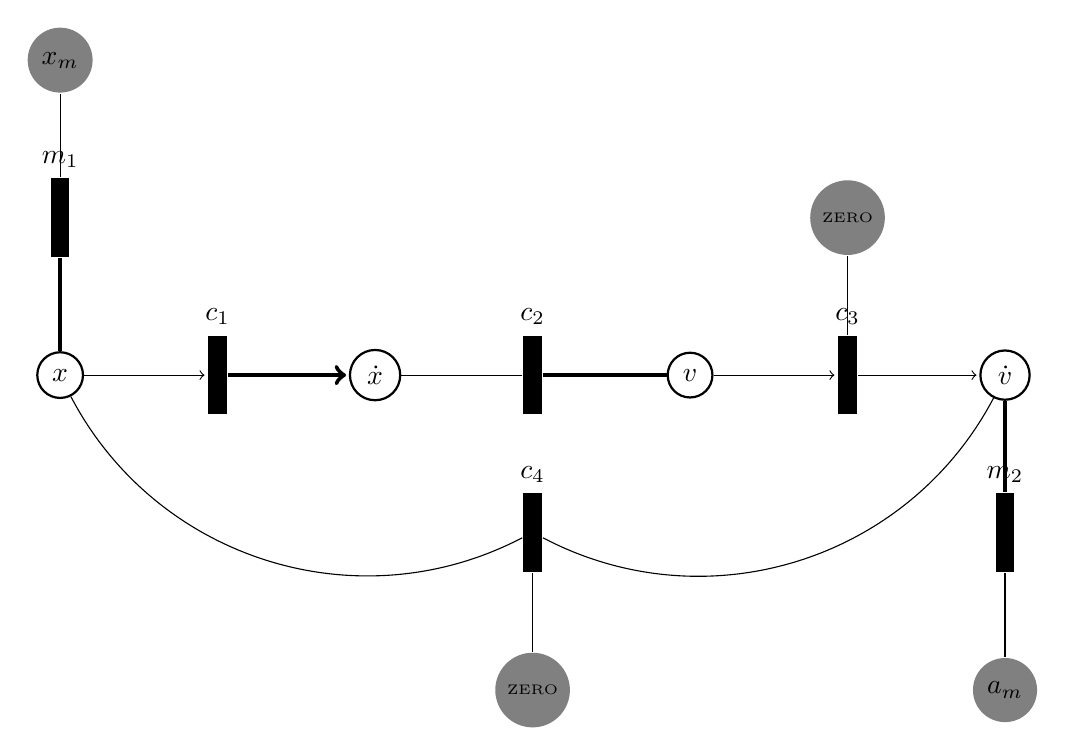
\begin{tikzpicture}[node distance = 2cm, bend angle=45, auto]
\tikzstyle{known_var}=[circle, thick,fill=gray]
\tikzstyle{unkno_var}=[circle, draw=black, thick]
\tikzstyle{constr}=[rectangle, fill=black, thick, minimum height=10mm, minimum width = 1mm]
%
\begin{scope}

\node [known_var] [](xm) {$x_m$};
\node [constr] (m1) [below of=xm,label=$m_1$] {}
	edge [] (xm);
\node [unkno_var] (x) [below of=m1] {$x$}
	edge [ultra thick] (m1);
\node [constr] (c1) [right of=x, label=$c_1$] {}
	edge [pre] (x);
\node [unkno_var] [right of=c1](xdot) {$\dot{x}$}
	edge [pre,ultra thick] (c1);
\node [constr] [right of=xdot, label=$c_2$] (c2) {}
	edge [] (xdot);
\node [unkno_var] [right of=c2] (v) {$v$}
	edge [ultra thick] (c2);
\node [constr] (c3) [right of=v, label=$c_3$] {}
	edge [pre] (v);
\node [unkno_var] [right of=c3] (vdot) {$\dot{v}$}
	edge [pre] (c3);
\node [constr] [below of=c2, label=$c_4$] (c4) {}
	edge [bend right] (vdot)
	edge [bend left] (x);
\node [known_var] [above of=c3] (zeroC3) {\tiny{ZERO}}
	edge [] (c3);
\node [constr] [below of=vdot, label=$m_2$] (m2) {}
	edge [ ultra thick] (vdot);
\node [known_var] [below of=m2] (am) {$a_m$}
	edge [] (m2);
\node [known_var] [below of=c4] (zeroC4) {\tiny{ZERO}}
	edge [] (c4);
\end{scope}
%
\end{tikzpicture}

The new Boolean mapping of the constraints onto the residuals is\\
$\begin{array}{c|cccccc}
	\>  & m_1 & m_2 & c_1 & c_2 & c_3 & c_4 \\ \hline
	r_1 &  1  &  1  &  1  &  1  &  1  &  0  \\
	r_2 &  1  &  1  &  0  &  0  &  0  &  1
\end{array}$

For demonstration purposes, if we assume that our sensors ($m_1$ and $m_2$) cannot fail, then the residual mapping will change to the one shown below and the spring-mass time constant fault can be isolated from differentiator faults.\\
$\begin{array}{c|cccc}
	\>  & c_1 & c_2 & c_3 & c_4 \\ \hline
	r_1 &  1  &  1  &  1  &  0  \\
	r_2 &  0  &  0  &  0  &  1
\end{array}$

Using this structured method, we can specify components-constraints whose faults we are interested to isolate, check their isolability properties formally and if there constraint is not isolable then possibly locate injection points where new sensors are needed to achieve isolability.

It would also be interesting to assign weights to each graph edge, in order to model the value of direct quantity measurements against quantities derived through extensive manipulation of the already known variables.

\clearpage
% UAV kinematics modeling
\chapter{Historical FDD Overview}

Fault Detection and Diagnosis is a subject of research since the end of the 70's, originally intended for application in the petrochemical industry, which was a very innovative, wealthy and large-scale sector at that time. Employing mainly state and parameter estimation techniques, which where very costly computationaly-wise at the time, FDD was barely applicable to the slow-evolving chemical processes.

During the 90's, when adaptive control was a new topic of interest, FDD was re-visited to aid in building fault-tolerant control systems. Especially in the airline industry, which at that time was both booming and employing in-flight computers with system-wide span, efforts where made to design systems which would automatically intervene to the pilot's actions, to detect some basic faults and avert potential (and potentially very expensive and life-threatening) accidents. However, the costly experimental iterations, as well as the inability to guarantee the correct operation of the fault-tolerant control system, which would in turn jeopardize human lives, prevented FDD and FTC from reaching their full potential in airborne systems.

UAVs provide the low-cost and disposable test platform which is needed to verify the efficiency of FDD methods and are getting increasing interest with every successful research milestone.
\clearpage
% UAV Dynamics modeling
\chapter{The Current FDD Scope w.r.t. Fixed-Wing UAVs}

The most fatal failure on a fixed-wing UAV (which have the traditional "airplane" shape), apart from severe structural damage, is a malfunction of its control surfaces. Indeed, an airplane could perform an emergency landing with malfunctioning undercarriage, with a reduced sensor suite, with a broken propeller or even without an engine. But without properly functioning ailerons and elevators the aircraft is essentially crippled. This is why most research in fw-UAV FDD revolves around detection of faults of control surfaces and their corresponding actuators.
Other research topics include detection of Pitot tube malfunctions and icing scenarios. The latter does not directly apply to consumer-grade UAVs, as the icing phenomenon occurs in high altitudes and low temperatures. The former has indeed applicable results to all fw-UAV airframes.
\clearpage
% Sensor modeling
\chapter{The Need for Holistic System Health Monitoring}

As is often quoted "The whole is more than the sum of its parts". In the case of fw-UAVs, the low-level system components have attributes and effects which not only affect themselves or the components they are connected to, but also the subsystem they belong to or even the whole airframe. Electrical, mechanical and dynamic interdependencies between components form a mesh of interactions, the knowledge of which is valuable. Each component is not isolated; its faults affect other parts of the system, even beyond its subsystem, and in turn said component may depend on other components working properly for itself to operate nominally. As an example, consider the case of an electric UAV, where a part of the propeller blade gets clipped, as a result of a hardware failure. Immediately, because of the imbalanced load on the motor shaft, the propeller angular inertia is increased and the motor struggles to maintain its commanded RPM. This results in excessive current draw and also reduced thrust power. Moreover, vibrations are generated and transmitted throughout the airframe, cluttering the accelerometer sensor bandwidth and possibly affecting the autopilot performance. Even in simple, single-component failures, the implications on a fast-evolving, tightly-coupled system may be severe and in ways that may not be directly apparent or so complex that are difficult to keep track of.

To showcase the extent of the problem, an indicative list of an UAV system resources and potential failures is presented.

\begin{table}[rc]
%\centering
\begin{minipage}[t]{0.45\textwidth}
\vspace{0pt}
\begin{tabular}{l}
{\textbf{System Resources}}\\
\hline
\underline{Hardware} \\
motor \\
actuators \\
sensors \\
video \& data tranceivers \\
antennae \\
fuel\\battery capacity \\
processing units (on-board computers) \\
aerodynamics surfaces \\
structural support \vspace{5pt}\\

\underline{Software} \\
Computational power \\
Computational memory \vspace{5pt} \\
\underline{Other}\\
Airspeed \\
Altitude
\end{tabular}
\end{minipage} %
%
\begin{minipage}[t]{0.45\textwidth}
\vspace{0pt}
\begin{tabular}{l}
{\textbf{System Faults}}\\
\hline
\underline{Hardware} \\
propeller damage \\
propeller dislocation \\
motor loss of power \\
motor total failure \\
power supply cut-off \\
power supply total failure \\
battery shortened life \\
battery fire \\
actuator failure \\
control surface dislocation\\
control surface break-off\\
sensor elevated noise floor \\
sensor failure\\
communication partial/total loss\\
structural failure partial/total\\
aerodynamic surface alteration\\
center of gravity dislocation \\
processor damage \vspace{5pt}\\
\underline{Software}\\
bugs\\
unexpected states
\end{tabular}
\end{minipage} %

\end{table}

It is apparent that in order to investigate the dependencies between system resources and system faults, with regard to component descriptions, we need to handle the system complexity using a formal, scalable representation method for this kind of dependencies.

\chapter{Other Future Directions}

\section{Residual Analysis}
Using formal ways to tackle large system complexity was shown to be beneficial for the purposes of Fault Detection and Diagnosis. In this text, the analysis ended with the production of residuals, which contain information on potential system faults. Inevitably, in order to extract final conclusions on system faults, these residuals have to be analyzed to recognize the appearance of fault signatures inside them. A plethora of methods is employed to achieve this goal, ranging from simple thresholding up to statistical tests and pattern recognition.

\section{Separating Faults from Disturbances}
Under the right system model, faults and disturbances can be handled in a similar fashion, and in the same ways that faults are detected and isolated and identified, so can disturbances be. This can prove beneficial for assessing the intensity of environmental disturbances.

\section{Hybrid Systems}
Hybrid systems have recently received a lot of attention in FDD and reconfigurable control applicaitons. Indeed, they offer an intuitive and formal way to handle events in the system, introduce temporal causality and define different system states, which in turn need different handling, in terms of monitoring, control and mission planning. Discrete Event Systems (DES) used along with the results from FMEA can also be used to back-track fault apparitions in time and have better estimates on fault isolation.

\section{Fault Identification and Reconfigurable/Restructurable Control}
If component failures can be precisely isolated, then the task of on-line system identification can be rendered a lot easier. If the system structure has not changed, then on-line identification algorithms can be focused on specific subsets of input/output signals to detect parameter changes with much greater accuracy. Thus adaptive controllers have an easier task to re-tune their gains for effective control. If structural changes are indeed detected, then this information can be used to perform re-structurable control.

\section{Mission Planning}
By having a constantly updated system structure/model, its limits and capabilities can be compared against mission goals to assess their feasibility in real-time. This not only adds an extra layer of safety for the UAV, since it enables it to abort un-achievable missions, but it may also enable it to re-specify its mission automatically in order to complete as much of the original mission as possible while being able to return to base at the same time.

%% APPENDICES %%%%%%%%%%%%%%%%%%%%%%%%%%%%%%%%%
\appendix


%% Bibliography Section %%%%%%%%%%%%%%%%%%%%%%%
\bibliographystyle{/home/georgezp/texmf/tex/bibtex/bst/plain.bst}
\bibliography{References,ReferencesModel}
%\printbibliography

\end{document}

